\chapter{The Standard Model of Particle Physics}
\label{chapter:SM}

%\epigraph{\textit{So it goes...}}{---Kurt Vonnegut, \textit{Slaughterhouse
%		Five}}
	
\epigraph{\textit{Ex pede Herculem. \newline(From the feet, Hercules.)}}{--Herodotus, Book IV, Section LXXXII. Plutarch}

%A deep understanding of something small in great details gives you understanding of everything else. 

%\epigraph{\textit{Quote}}{--Unknown, \textit{}}
%\epigraph{\textit{Quote}}{--Person}


\section{Description}
The Standard Model of Particle Physics is the epitome of human understanding of elementary building blocks of the physical world and to date. It lays out seventeen particles, their properties, and interactions, in the three fundamental forces, the electromagnetic, the weak, and the strong force. Everyday movements, from flipping the page of a book, to transportation; from weak beta decay in atomic decay to interaction of quarks within an atom nucleus, can be described by Stanard Model
particles and their interactions.

The Standard Model of Particle Physics is a gauge theory under the quantum field theory framework. Particles are represented different quantized fields operators. The particle interactions are determined by the standard model Lagrangian. Like other physic theories, the Lagrangian of the Standard Model observes physics symmetries.

\subsection*{Symmetry}
    Symmetry is the foundation of many laws in physics including the standard model. The Noether's Theorem has elegantly linked different symmetries to different conserved quantities:

    %\begin{description}[font=$\bullet$~\normalfont\scshape\color{black!50!black}]
    %\begin{itemize}
    %    \item Spatial Translational Symmetry $\rightarrow$ Translational Momentum Conservation

    %    \item Time Symmetry $\rightarrow$ Energy Conservation

    %    \item Rotational Symmetry $\rightarrow$ Angular Momentum Conservation

    %\end{itemize}

Following from the Special Relativity, the invariance applies to all observers in different frames, and the above three can be summarized by the Lorentz symmetry ($\mathcal{P}$) and a transformation in the Lorentz group. The invariance quantity under this transformation is called the Lorentz invariance. 
    Apart from the Lorentz invariance, the Standard Model also observes internal local symmetries between particles. Namely  \SUthree$_C \times $ \SUtwo$_L \times$\Uone$_{Y}$, these internal symmetries describe the particle interactions and as "transformations" between different particles, owing to the property of a gauge theory, these transformations are mediated by mediator particles. The different physical invariant quantities that are conserved under these particle
    transformation/interactions are called "charges", their interactions processes are sometimes called "currents".

    The influence of the individual part of the internal symmetries are described as follows: The local $SU(3)_{C}$ symmetry governs the strong force and only has an effect on particles with a color charge (either red, green, or blue). These particles in the Standard Model include quarks of field $\mathcal{Q}_{i}$, which include the left-handed doublets of ($u_{L}$, $d_{L}$), ($c_{L}$, $s_{L}$), ($t_{L}$, $b_{L}$). The symmetry also affects quark fields of right-handed singlets of $u_{R,i}$ and $d_{R}$. The strong force is mediated by the eight gluon fields $\mathcal{G}$.

    %[Rewrite this paragraph]
    The $SU(2)_{L}$ transformation describes the weak force and is effective on particles with the weak charge, it is mediated by three W bosons ($W_{1}$,$W_{2}$,$W_{3}$), the \Uone transformation is mediated by the weak boson B and acts on particles that has a weak hyper-charge Y. The combined effect of the weak field and the weak hyper-charge field give us the familiar electro-magnetic weak force in day-to-day (including the LHC) energy scale below the spontaneous symmetry breaking, and has an effect on most quark fields, bosons, as well as leptonic fields, which include the lepton field of left-handed doublets of ($e_{L}$, $\nu_{e,L}$), ($\mu_{L}$, $\nu_{\mu,L}$), ($\tau_{L}$, $\nu_{\tau,L}$) and the right-handed singlets of $e_{R}$, $\mu_{R}$, and $\tau_{R}$.

    %[What are the charges? and how does it form the normal charges.]
    
    %The combined effect of the $SU(2)_L \times U(1)_{Y}$ gives us the familiar effect of electromagnetism/weak force effect below the spontaneous symmetry breaking scale, and affect the Q field described above, as well as the leptonic field of \mathcal{L}$_{i}$ 

\begin{table}[!htb]
    \begin{center}
        \begin{tabularx}{0.8\textwidth}{m{1em} c c c c c c c }
        \toprule
        \hline
& Field & Members & Spin & \Uone$_{Y}$) & \SUtwo$_{L}$ & \SUthree$_{C}$ \\
        \hline

        %\rotatebox{90}{\hspace{-0.1cm}\textbf{Fermionic Field} }
            \rotatebox{90}{\hspace{-0.1cm}\textbf{Leptons} }
             &   \makecell{\fieldLi \\ \fieldEri} % FIELD
             &   \makecell{ (\fieldEl, \fieldNuEl), (\fieldMul, \fieldNuMul), (\fieldTaul, \fieldNuTaul) \\ \fieldEr, \fieldMur, \fieldTaur}% CONTENT
             &   \makecell{ $1/2$ \\ $1/2$ }% SPIN
             &   \makecell{ $-1$ \\ $-2$ }% U(1)
             &   \makecell{ $\mathbf{2}$ \\ $\mathbf{1}$ }% SU(2)
             &   \makecell{ $\mathbf{1}$ \\ $\mathbf{1}$ } \\ % SU(3)
            \midrule
            \rotatebox{90}{\hspace{-0.1cm}\textbf{Quarks} } 
             &   \makecell{\fieldQi \\ \fieldUri \\ \fieldDri} % FIELD
             &   \makecell{ (\fieldUl, \fieldDl), (\fieldCl, \fieldSl), (\fieldTl, \fieldBl) \\ \fieldUr \\ \fieldDr}% CONTENT
             &   \makecell{ $1/2$ \\ $1/2$ \\ $1/2$} % SPIN
             &   \makecell{ $1/3$ \\ $4/3$ \\ $-2/3$}% U(1)
             &   \makecell{ $\mathbf{2}$ \\ $\mathbf{1}$ \\ $\mathbf{1}$}% SU(2)
             &   \makecell{ $\mathbf{3}$ \\ $\mathbf{3}$ \\ $\mathbf{3}$}\\ % SU(3)

        \cdashline{1-7}

        %\rotatebox{90}{\hspace{-0.1cm}\textbf{Bosonic Field} }
            \rotatebox{90}{\textbf{\stackanchor{Gauge}{Fields}} }
             &   \makecell{\fieldB \\ \fieldW \\ \fieldG } % FIELD
             &   \makecell{ \fieldB \\ (\fieldWone, \fieldWtwo, \fieldWthree) \\ \fieldG$_a$, $a\in[1,..,8]$ }% CONTENT
             &   \makecell{ $1$ \\ $1$ \\ $1$} % SPIN
             &   \makecell{ $0$ \\ $0$ \\ $0$}% U(1)
             &   \makecell{ $\mathbf{1}$ \\ $\mathbf{3}$ \\ $\mathbf{1}$}% SU(2)
             &   \makecell{ $\mathbf{1}$ \\ $\mathbf{1}$ \\ $\mathbf{8}$}\\ % SU(3)
            \midrule
            \rotatebox{90}{\textbf{\stackanchor{Higgs}{Field}}} 
             &   \makecell{\fieldPhi } % FIELD
             &   \makecell{ (\fieldPhip, \fieldPhizero) }% CONTENT
             &   \makecell{ $0$  } % SPIN
             &   \makecell{ $1$  }% U(1)
             &   \makecell{ $\mathbf{2}$ }% SU(2)
             &   \makecell{ $\mathbf{1}$ }\\ % SU(3)
        \hline
        \bottomrule
        \end{tabularx}
    \end{center}

    \caption{
        The particle fields of the SM\cite{Antrim:2699575}.
    \label{table:sm1}
    }

\end{table}

\FloatBarrier


A detailed list of the gauge fields field and their charges along with their mathematical group can be found in table~\ref{table:sm}~\cite{Antrim:2699575}. 

\subsection*{Spontaneous Symmetry Breaking}
The standard model theory in the form as presented in the last section does not give mass to the particles, this is inconsistent with observation in experiment. The process of giving mass to the particle process is called the spontaneous symmetry breaking process.
[More details later]
%A scalar field with the name of the Higgs field, is coupled to the \SUtwo$_L$ \times \Uone$_Y$ group weak-hyper charge. The potential of the field has the shape of a Mexican hat, 


\begin{table}[!htb]
    \caption{
        The table shows the particle fields of the SM after SSB. Coupling and mass parameters are provided. 
    }
        %The particle content of the SM after the process of
        %electroweak symmetry breaking.
        %Shown for each particle species are the associated electric charge, $Q$,
        %coupling, and mass (approximate).
        %The $y_i$ are the Yukawa coupling (Equation~\ref{eq:higgs_fermion_coupling}),
        %$\alpha_{\text{EM}}$ is the QED coupling constant (`fine structure constant'),
        %$\mathcal{V}$ indicates the parameters of the CKM matrix, and
        %$\alpha_s$ is the QCD coupling constant.
        %The quantities $\lambda$ and $\mu$ are the Higgs self-coupling parameter
        %and mass terms, respectively, appearing in Higgs potential terms (Equation~\ref{eq:higgs_potential}).
    \begin{center}
        \begin{tabularx}{1\textwidth}{m{1em} c c c c }
        \toprule
        \hline
        & Physical Field & Q & Coupling & Mass [GeV] \\
        \hline
        \rotatebox{90}{\hspace{-0.1cm}\textbf{Quarks} } 
            & \makecell{ \quarkU, \quarkC, \quarkT \\ \quarkD, \quarkS, \quarkB} % FIELD
            & \makecell{ $2/3$ \\ $-1/3$ }% Q
            %& \makecell{ $\mathbf{3}$ \\ $\mathbf{3}$ } % SU(3)
            & \makecell{ ($y_i=$) $1\times10^{-5}$, $7\times10^{-3}$, $1$ \\ ($y_i=$) $3\times10^{-5}$, $5\times10^{-4}$, $0.02$ } % Coupling
            & \makecell{ $2\times10^{-3}$, $1.27$, $173$ \\ $4\times10^{-4}$, $0.10$, $4.18$ }\\% Mass
        \rotatebox{90}{\hspace{-0.1cm}\textbf{Leptons} } 
            & \makecell{ \leptonE, \leptonMu, \leptonTau \\ \neutrinoE, \neutrinoMu, \neutrinoTau } % FIELD
            & \makecell{ $-1$ \\ $0$ }% Q
            %& \makecell{ $\mathbf{1}$ \\ $\mathbf{1}$ } % SU(3)
            & \makecell{ ($y_i=$) $3\times10^{-7}$, $6\times10^{-4}$, $0.01$ \\ -- } % Coupling
            & \makecell{ $5\times10^{-4}$, $0.106$, $1.777$ \\ --}\\% Mass
        \midrule
        \rotatebox{90}{\textbf{Bosons} } 
            & \makecell{ \fieldPhoton \\ \fieldZ \\ (\fieldWp, \fieldWm) \\ \fieldG } % FIELD
            & \makecell{ $0$ \\ $0$ \\ $(+1,-1)$ \\ $0$ }% Q
            %& \makecell{ $\mathbf{1}$ \\ $\mathbf{1}$ \\ $\mathbf{1}$ \\ $\mathbf{8}$ } % SU(3)
            & \makecell{ $\alpha_{\text{EM}} \simeq 1/137$ \\ $\sin \theta_{W} \simeq 0.5$ \\ $\mathcal{V}_{\text{CKM}}$ \\ $\alpha_s \simeq 0.1$ } % Coupling
            & \makecell{ $0$ \\ $91.2$ \\ $80.4$ \\  $0$}\\% Mass
        \midrule
        \rotatebox{90}{\textbf{Higgs} } 
            & \makecell{ \fieldH } % FIELD
            & \makecell{ $0$ }% Q
            %& \makecell{ $\mathbf{1}$ } % SU(3)
            & \makecell{ $\lambda$, $\mu$ } % Coupling
            & \makecell{ $125.09$ }\\% Mass
        \hline
        \bottomrule
        \end{tabularx}
    \end{center}
    \label{tab:sm_content_EWSB}
\end{table}


After spontaneous symmetry breaking, the physical field and their measured properties take the following form~\ref{tab:sm_content_EWSB}:
    
    The complete Standard Model Lagrangian can be represented as follows:

%\begin{equation}
%\begin{center}
%\begin{math}
%-\frac{1}{2}\partial_{\nu}g^{a}_{\mu}\partial_{\nu}g^{a}_{\mu}
%-g_{s}f^{abc}\partial_{\mu}g^{a}_{\nu}g^{b}_{\mu}g^{c}_{\nu}
%-\frac{1}{4}g^{2}_{s}f^{abc}f^{ade}g^{b}_{\mu}g^{c}_{\nu}g^{d}_{\mu}g^{e}_{\nu}
%+\frac{1}{2}ig^{2}_{s}(\bar{q}^{\sigma}_{i}\gamma^{\mu}q^{\sigma}_{j})g^{a}_{\mu}
%+\bar{G}^{a}\partial^{2}G^{a}+g_{s}f^{abc}\partial_{\mu}\bar{G}^{a}G^{b}g^{c}_{\mu}
%-\partial_{\nu}W^{+}_{\mu}\partial_{\nu}W^{-}_{\mu}-M^{2}W^{+}_{\mu}W^{-}_{\mu}
%-\frac{1}{2}\partial_{\nu}Z^{0}_{\mu}\partial_{\nu}Z^{0}_{\mu}-\frac{1}{2c^{2}_{w}}
%M^{2}Z^{0}_{\mu}Z^{0}_{\mu}
%-\frac{1}{2}\partial_{\mu}A_{\nu}\partial_{\mu}A_{\nu}
%-\frac{1}{2}\partial_{\mu}H\partial_{\mu}H-\frac{1}{2}m^{2}_{h}H^{2}
%-\partial_{\mu}\phi^{+}\partial_{\mu}\phi^{-}-M^{2}\phi^{+}\phi^{-}
%-\frac{1}{2}\partial_{\mu}\phi^{0}\partial_{\mu}\phi^{0}-\frac{1}{2c^{2}_{w}}M\phi^{0}\phi^{0}
%-\beta_{h}[\frac{2M^{2}}{g^{2}}+\frac{2M}{g}H+\frac{1}{2}(H^{2}+\phi^{0}\phi^{0}+2\phi^{+}\phi^{-%%@
%})]+\frac{2M^{4}}{g^{2}}\alpha_{h}
%-igc_{w}[\partial_{\nu}Z^{0}_{\mu}(W^{+}_{\mu}W^{-}_{\nu}-W^{+}_{\nu}W^{-}_{\mu})
%-Z^{0}_{\nu}(W^{+}_{\mu}\partial_{\nu}W^{-}_{\mu}-W^{-}_{\mu}\partial_{\nu}W^{+}_{\mu})
%+Z^{0}_{\mu}(W^{+}_{\nu}\partial_{\nu}W^{-}_{\mu}-W^{-}_{\nu}\partial_{\nu}W^{+}_{\mu})]
%-igs_{w}[\partial_{\nu}A_{\mu}(W^{+}_{\mu}W^{-}_{\nu}-W^{+}_{\nu}W^{-}_{\mu})
%-A_{\nu}(W^{+}_{\mu}\partial_{\nu}W^{-}_{\mu}-W^{-}_{\mu}\partial_{\nu}W^{+}_{\mu})
%+A_{\mu}(W^{+}_{\nu}\partial_{\nu}W^{-}_{\mu}-W^{-}_{\nu}\partial_{\nu}W^{+}_{\mu})]
%-\frac{1}{2}g^{2}W^{+}_{\mu}W^{-}_{\mu}W^{+}_{\nu}W^{-}_{\nu}+\frac{1}{2}g^{2}
%W^{+}_{\mu}W^{-}_{\nu}W^{+}_{\mu}W^{-}_{\nu}
%+g^2c^{2}_{w}(Z^{0}_{\mu}W^{+}_{\mu}Z^{0}_{\nu}W^{-}_{\nu}-Z^{0}_{\mu}Z^{0}_{\mu}W^{+}_{\nu}
%W^{-}_{\nu})
%+g^2s^{2}_{w}(A_{\mu}W^{+}_{\mu}A_{\nu}W^{-}_{\nu}-A_{\mu}A_{\mu}W^{+}_{\nu}
%W^{-}_{\nu})
%+g^{2}s_{w}c_{w}[A_{\mu}Z^{0}_{\nu}(W^{+}_{\mu}W^{-}_{\nu}-W^{+}_{\nu}W^{-}_{\mu})-%%@
%2A_{\mu}Z^{0}_{\mu}W^{+}_{\nu}W^{-}_{\nu}]
%-g\alpha[H^3+H\phi^{0}\phi^{0}+2H\phi^{+}\phi^{-}]
%-\frac{1}{8}g^{2}\alpha_{h}[H^4+(\phi^{0})^{4}+4(\phi^{+}\phi^{-})^{2}+4(\phi^{0})^{2}
%\phi^{+}\phi^{-}+4H^{2}\phi^{+}\phi^{-}+2(\phi^{0})^{2}H^{2}]
%-gMW^{+}_{\mu}W^{-}_{\mu}H-\frac{1}{2}g\frac{M}{c^{2}_{w}}Z^{0}_{\mu}Z^{0}_{\mu}H
%-\frac{1}{2}ig[W^{+}_{\mu}(\phi^{0}\partial_{\mu}\phi^{-}-\phi^{-}\partial_{\mu}\phi^{0})
%-W^{-}_{\mu}(\phi^{0}\partial_{\mu}\phi^{+}-\phi^{+}\partial_{\mu}\phi^{0})]
%+\frac{1}{2}g[W^{+}_{\mu}(H\partial_{\mu}\phi^{-}-\phi^{-}\partial_{\mu}H)
%-W^{-}_{\mu}(H\partial_{\mu}\phi^{+}-\phi^{+}\partial_{\mu}H)]
%+\frac{1}{2}g\frac{1}{c_{w}}(Z^{0}_{\mu}(H\partial_{\mu}\phi^{0}-\phi^{0}\partial_{\mu}H)
%-ig\frac{s^{2}_{w}}{c_{w}}MZ^{0}_{\mu}(W^{+}_{\mu}\phi^{-}-W^{-}_{\mu}\phi^{+})
%+igs_{w}MA_{\mu}(W^{+}_{\mu}\phi^{-}-W^{-}_{\mu}\phi^{+})
%-ig\frac{1-2c^{2}_{w}}{2c_{w}}Z^{0}_{\mu}(\phi^{+}\partial_{\mu}\phi^{-}-\phi^{-%%@
%}\partial_{\mu}\phi^{+})
%+igs_{w}A_{\mu}(\phi^{+}\partial_{\mu}\phi^{-}-\phi^{-}\partial_{\mu}\phi^{+})
%-\frac{1}{4}g^{2}W^{+}_{\mu}W^{-}_{\mu}[H^{2}+(\phi^{0})^{2}+2\phi^{+}\phi^{-}]
%-\frac{1}{4}g^{2}\frac{1}{c^{2}_{w}}Z^{0}_{\mu}Z^{0}_{\mu}[H^{2}+(\phi^{0})^{2}+2(2s^{2}_{w}-%%@
%1)^{2}\phi^{+}\phi^{-}]
%-\frac{1}{2}g^{2}\frac{s^{2}_{w}}{c_{w}}Z^{0}_{\mu}\phi^{0}(W^{+}_{\mu}\phi^{-}+W^{-%%@
%}_{\mu}\phi^{+})
%-\frac{1}{2}ig^{2}\frac{s^{2}_{w}}{c_{w}}Z^{0}_{\mu}H(W^{+}_{\mu}\phi^{-}-W^{-}_{\mu}\phi^{+})
%+\frac{1}{2}g^{2}s_{w}A_{\mu}\phi^{0}(W^{+}_{\mu}\phi^{-}+W^{-}_{\mu}\phi^{+})
%+\frac{1}{2}ig^{2}s_{w}A_{\mu}H(W^{+}_{\mu}\phi^{-}-W^{-}_{\mu}\phi^{+})
%-g^{2}\frac{s_{w}}{c_{w}}(2c^{2}_{w}-1)Z^{0}_{\mu}A_{\mu}\phi^{+}\phi^{-}-%%@
%g^{1}s^{2}_{w}A_{\mu}A_{\mu}\phi^{+}\phi^{-}
%-\bar{e}^{\lambda}(\gamma\partial+m^{\lambda}_{e})e^{\lambda}
%-\bar{\nu}^{\lambda}\gamma\partial\nu^{\lambda}
%-\bar{u}^{\lambda}_{j}(\gamma\partial+m^{\lambda}_{u})u^{\lambda}_{j}
%-\bar{d}^{\lambda}_{j}(\gamma\partial+m^{\lambda}_{d})d^{\lambda}_{j}
%+igs_{w}A_{\mu}[-(\bar{e}^{\lambda}\gamma^{\mu}
%e^{\lambda})+\frac{2}{3}(\bar{u}^{\lambda}_{j}\gamma^{\mu} %%@
%u^{\lambda}_{j})-\frac{1}{3}(\bar{d}^{\lambda}_{j}\gamma^{\mu} 
%d^{\lambda}_{j})]
%+\frac{ig}{4c_{w}}Z^{0}_{\mu}
%[(\bar{\nu}^{\lambda}\gamma^{\mu}(1+\gamma^{5})\nu^{\lambda})+
%(\bar{e}^{\lambda}\gamma^{\mu}(4s^{2}_{w}-1-\gamma^{5})e^{\lambda})+
%(\bar{u}^{\lambda}_{j}\gamma^{\mu}(\frac{4}{3}s^{2}_{w}-1-\gamma^{5})u^{\lambda}_{j})+
%(\bar{d}^{\lambda}_{j}\gamma^{\mu}(1-\frac{8}{3}s^{2}_{w}-\gamma^{5})d^{\lambda}_{j})]
%+\frac{ig}{2\sqrt{2}}W^{+}_{\mu}[(\bar{\nu}^{\lambda}\gamma^{\mu}(1+\gamma^{5})e^{\lambda})
%+(\bar{u}^{\lambda}_{j}\gamma^{\mu}(1+\gamma^{5})C_{\lambda\kappa}d^{\kappa}_{j})]
%+\frac{ig}{2\sqrt{2}}W^{-}_{\mu}[(\bar{e}^{\lambda}\gamma^{\mu}(1+\gamma^{5})\nu^{\lambda})
%+(\bar{d}^{\kappa}_{j}C^{\dagger}_{\lambda\kappa}\gamma^{\mu}(1+\gamma^{5})u^{\lambda}_{j})]
%+\frac{ig}{2\sqrt{2}}\frac{m^{\lambda}_{e}}{M}
%[-\phi^{+}(\bar{\nu}^{\lambda}(1-\gamma^{5})e^{\lambda})
%+\phi^{-}(\bar{e}^{\lambda}(1+\gamma^{5})\nu^{\lambda})]
%-\frac{g}{2}\frac{m^{\lambda}_{e}}{M}[H(\bar{e}^{\lambda}e^{\lambda})
%+i\phi^{0}(\bar{e}^{\lambda}\gamma^{5}e^{\lambda})]
%+\frac{ig}{2M\sqrt{2}}\phi^{+}
%[-m^{\kappa}_{d}(\bar{u}^{\lambda}_{j}C_{\lambda\kappa}(1-\gamma^{5})d^{\kappa}_{j})
%+m^{\lambda}_{u}(\bar{u}^{\lambda}_{j}C_{\lambda\kappa}(1+\gamma^{5})d^{\kappa}_{j}]
%+\frac{ig}{2M\sqrt{2}}\phi^{-}
%[m^{\lambda}_{d}(\bar{d}^{\lambda}_{j}C^{\dagger}_{\lambda\kappa}(1+\gamma^{5})u^{\kappa}_{j})
%-m^{\kappa}_{u}(\bar{d}^{\lambda}_{j}C^{\dagger}_{\lambda\kappa}(1-\gamma^{5})u^{\kappa}_{j}]
%-\frac{g}{2}\frac{m^{\lambda}_{u}}{M}H(\bar{u}^{\lambda}_{j}u^{\lambda}_{j})
%-\frac{g}{2}\frac{m^{\lambda}_{d}}{M}H(\bar{d}^{\lambda}_{j}d^{\lambda}_{j})
%+\frac{ig}{2}\frac{m^{\lambda}_{u}}{M}\phi^{0}(\bar{u}^{\lambda}_{j}\gamma^{5}u^{\lambda}_{j})
%-\frac{ig}{2}\frac{m^{\lambda}_{d}}{M}\phi^{0}(\bar{d}^{\lambda}_{j}\gamma^{5}d^{\lambda}_{j})
%+\bar{X}^{+}(\partial^{2}-M^{2})X^{+}+\bar{X}^{-}(\partial^{2}-M^{2})X^{-}
%+\bar{X}^{0}(\partial^{2}-\frac{M^{2}}{c^{2}_{w}})X^{0}+\bar{Y}\partial^{2}Y
%+igc_{w}W^{+}_{\mu}(\partial_{\mu}\bar{X}^{0}X^{-}-\partial_{\mu}\bar{X}^{+}X^{0})
%+igs_{w}W^{+}_{\mu}(\partial_{\mu}\bar{Y}X^{-}-\partial_{\mu}\bar{X}^{+}Y)
%+igc_{w}W^{-}_{\mu}(\partial_{\mu}\bar{X}^{-}X^{0}-\partial_{\mu}\bar{X}^{0}X^{+})
%+igs_{w}W^{-}_{\mu}(\partial_{\mu}\bar{X}^{-}Y-\partial_{\mu}\bar{Y}X^{+})
%+igc_{w}Z^{0}_{\mu}(\partial_{\mu}\bar{X}^{+}X^{+}-\partial_{\mu}\bar{X}^{-}X^{-})
%+igs_{w}A_{\mu}(\partial_{\mu}\bar{X}^{+}X^{+}-\partial_{\mu}\bar{X}^{-}X^{-})
%-\frac{1}{2}gM[\bar{X}^{+}X^{+}H+\bar{X}^{-}X^{-}H+\frac{1}{c^{2}_{w}}\bar{X}^{0}X^{0}H]
%+\frac{1-2c^{2}_{w}}{2c_{w}}igM[\bar{X}^{+}X^{0}\phi^{+}-\bar{X}^{-}X^{0}\phi^{-}]
%+\frac{1}{2c_{w}}igM[\bar{X}^{0}X^{-}\phi^{+}-\bar{X}^{0}X^{+}\phi^{-}]
%+igMs_{w}[\bar{X}^{0}X^{-}\phi^{+}-\bar{X}^{0}X^{+}\phi^{-}]
%+\frac{1}{2}igM[\bar{X}^{+}X^{+}\phi^{0}-\bar{X}^{-}X^{-}\phi^{0}]
%\end{math}
%\end{center}    
%\label{eq:SM}
%\end{equation}

    %TODO how to cite this ?

%\begin{align*}

%\begin{equation}
%\begin{aligned}
%	\mathcal{L} = &-\frac{1}{4} B_{\mu\nu}B^{\mu\nu} - \frac{1}{8}tr\left(\mathbf{W}_{\mu\nu}\mathbf{W}^{\mu\nu}\right) - \frac{1}{2}tr\left(\mathbf{G}_{\mu\nu}\mathbf{G}^{\mu\nu}\right) 
%    \\ \text{(U(1), SU(2), and SU(3) gauge terms)} \\
%    LALA
%	%&+ \left(\bar{\nu}_L,\bar{e}_L\right)\tilde{\sigma}^\mu iD_\mu\icol{\nu_L\\e_L} + \bar{e}_R\sigma^\mu iD_\mu e_R + \bar{\nu}_R\sigma^\mu iD_\mu\nu_R + \text{(h.c.)} && \text{(lepton dynamical term)} \\
%	%&-\frac{\sqrt{2}}{\nu}\left[\left(\bar{\nu}_L,\bar{e}_L\right)\phi M^ee_R+\bar{e}_R\bar{M}^e\bar{\phi}\icol{\nu_L\\e_L}\right] && \text{(electron, muon, tauon mass term)} \\
%	%&-\frac{\sqrt{2}}{\nu}\left[\left(-\bar{e}_L,\bar{\nu}_L\right)\phi^{*}M^\nu\nu_R+\bar{\nu}_R\bar{M}^\nu\phi^T\icol{-e_L\\\nu_L}\right] && \text{(neutrino mass term)} \\
%	%& +\left(\bar{u}_L, \bar{d}_L\right)\tilde{\sigma}^\mu iD_\mu \icol{u_L\\d_L} + \bar{u}_R\sigma^\mu iD_\mu u_R + \bar{d}_R\sigma^\mu iD_\mu d_R + \text{(h.c.)} && \text{(quark dynamical term)} \\
%	%&- \frac{\sqrt{2}}{\nu}\left[\left(\bar{u}_L,\bar{d}_L\right)\phi M^dd_R+\bar{d}_R\bar{M}^d\bar{\phi}\icol{u_L\\d_L}\right] && \text{(down, strange, bottom mass term)} \\
%	%&-\frac{\sqrt{2}}{\nu}\left[\left(-\bar{d}_L,\bar{u}_L\right)\phi^{*}M^uu_R+\bar{u}_R\bar{M}^u\phi^T\icol{-d_L\\u_L}\right] && \text{(up, charm, top mass term)} \\
%	%&+\overline{\left(D_\mu\phi\right)}D^\mu\phi-\frac{m_h^2\left[\bar{\phi}\phi-\frac{\nu^2}{2}\right]^2}{2\nu^2} && \text{(Higgs dynamical and mass term)}
%
%
%\begin{aligned}
%\label{eq:SM}
%\end{equation}
%%\end{align*} 
%

%    These field represent threpresents three out of four of the fundamental forces, the weak, the electromagnetic and the strong force.
%    Under the usual scale of everyday life and in the scale of the experiment, spontaneous symmetry breaking lead to Goldstone bosons gaining mass from their original field, a total of seventeen particles are observed.
    The Standard Model lagrangian contains seventeen particles along with their anti-particle counterparts. There are two types of particles, the bosons, and the fermions: The bosons are particles that have integer spin and can be described by the Einstein-Bose statistics. They include the force mediator particles, like photon, W+-, Z bosons and a particle predicted by the Brout-Englert-Higgs mechanism, the Higgs boson; The fermions are particles that contain half spins, they include the quark
     and leptons, they are each divided into three generations. While only the quarks are influenced by the strong force, both types of these particles are influenced by the electro-weak force.

     A complete list of the experimentally accessible particles can be found here in table~\ref{table:sm_content_EWSB}:

    \begin{figure}[!htb]
        \begin{center}
            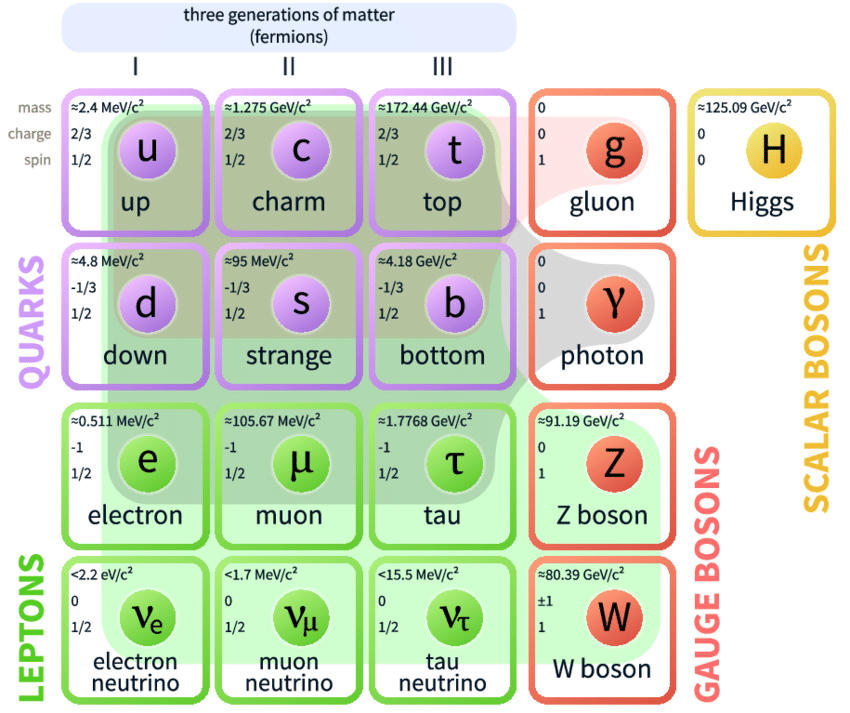
\includegraphics[width=0.75\textwidth]{figures/chapter_SM/SM}
            \caption{
                A schematic diagram of the Standard Model Particles seen in the scale of the experiment of the Large Hadron Collider.
            }
            \label{fig:SM}
        \end{center}
    \end{figure}

\section{Sucessful Prediction}
The Standard Model has many successes in the particle level, and it has made along with many successful predictions, these predictions include:
    \begin{itemize}
        \item existence of W boson %~\cite{}
        \item existence of Z boson %~\cite{}
        \item existence of the charm quark %~\cite{}
        \item existence of the top quark %~\cite{}
        \item existence of the Higgs boson %~\cite{}
    \end{itemize}

\section{Standard Model Measurement}
Many Standard Model properties has been measured under the ATLAS experiment, a summary plot on the cross section of the interactions can be found here:
%Summary plots 

    \begin{figure}[!htb]
        \begin{center}
            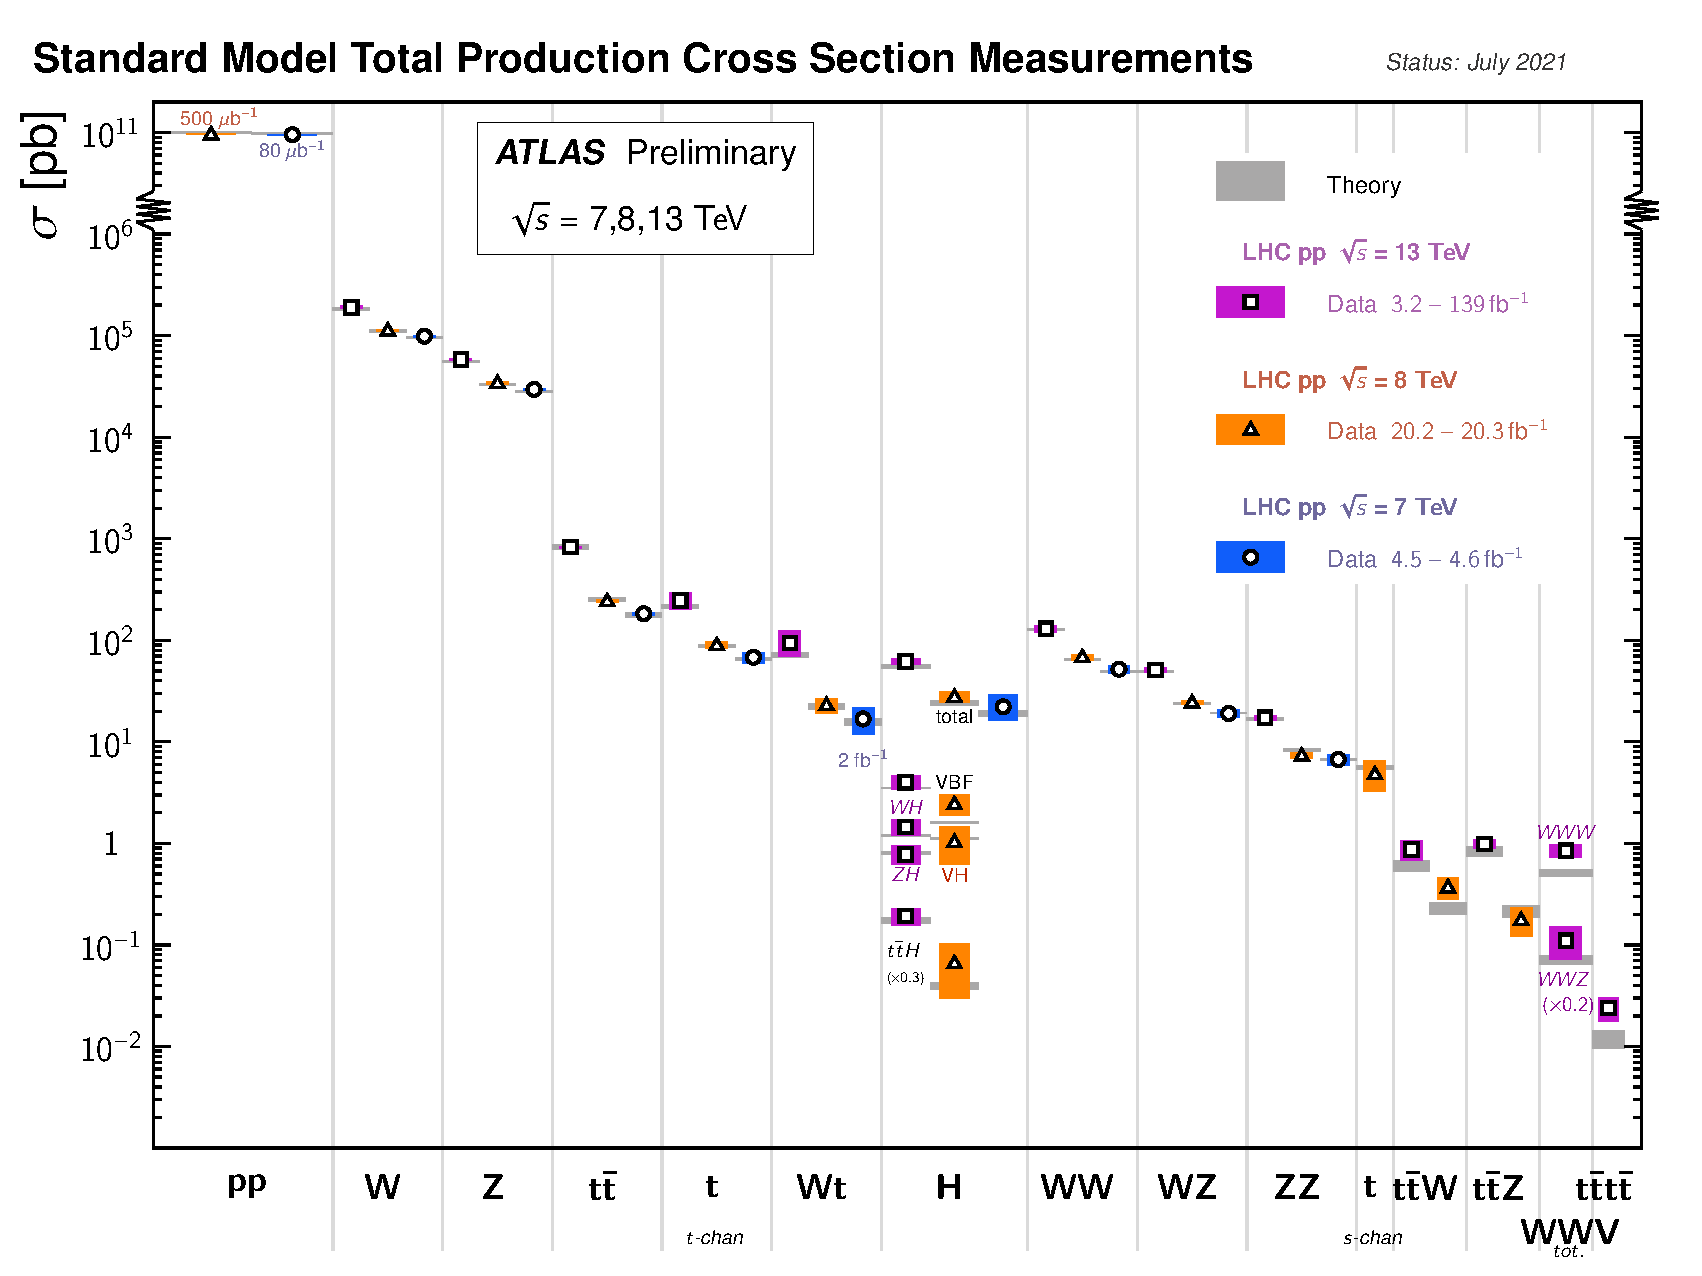
\includegraphics[width=0.75\textwidth]{figures/chapter_SM/SM_Measurement}
            \caption{
                A summary plot on the Standard Model cross-section measurements done by the ATLAS experiment~\cite{ATL-PHYS-PUB-2021-032}.
            }
            \label{fig:SM}

        \end{center}
    \end{figure}



\section{Unresolved Problems in the Standard Model}
The Standard Model of Particle Physics in its current forms has had many standing unresolved problems, leading to the belief that the model, despite its many successes is not the ultimate theory on fundamental particles. Here, some of the standing problems of the standard model and their proposed solutions are discussed.

\subsection{Gravity}
The Standard Model does not include gravity, one of four fundamental forces.     

\subsection{Naturalness}
Naturalness is the property in physics theory where the dimensionless ratio between the free parameters and the physical constants should be in the order of 1. When a physical theory takes either a very large or small value outside the order of 1, they are considered unnatural and unlikely to be the fundamental theory. 
The Standard Model shows many naturalness issues in different dimensions: 

\subsubsection{The Cosmological Constant Problem}
The Standard Model allows for a 0th dimension constant in its Lagrangian that would not break any of its symmetries. The constant would represent the vacuum energy density and would account for the quantum fluctuation in vacuum. Under Zelokoch's calculations~\cite{zel1968cosmological}, the relations between the vacuum energy density and the cosmological constant of the Einstein's Equation is directly proportional as such:

\begin{equation}
    \rho_{vac}c^2=\Lambda c^4/8\pi G
\label{eq:cosmoconst}
\end{equation}

The cosmological constant is a well-measured value in cosmology from the measurement of the expansion of the universe. The cutting off in either the Planck scale or the electro-weak scale in quantum field theory gives a theoretical prediction value of the vacuum expectation value. However, these values do not match. The experimental measured value of $\rho_{vac}$ is about 40-100 more order of magnitude smaller than what's predicted in theory. The order of magnitude discrepancy poses the
biggest naturalness issue in the Standard Model~\cite{V2002}.

%Currently, there are proposition that the discrepany could be due to the fact that the neighboring universe is antropologically different than the whole universe[], or modifications could be done to the Einstein's Equation. But as these propositions violates other universal principle or theorems, none are satisfactory.


%In cosmology, it's known that there is a vacuum energy density that exist in the curvature of the universe that can be expressed as the cosmological constant in the Einstein's Equation. The Cosmological constant is measured with the expansion of the universe and would convert to a vacuum 
%In the 0th order, the cosmological constant as measured by experiment is between 40-100 more order of magniture smaller than predicted. 


\subsubsection{The Higgs Hierarchy Problem}
The Higgs hierarchy problem of particle physics describes the apparent large discrepancy in order of magnitude between the electro-weak scale and the gravitational scale, the weak force is about $10^{24}$ greater than gravity. Its effect can be seen in the Higgs mass boson as the mass is 17 order smaller than would be expected by the Planck mass. 
A popular solution is quantum corrections via supersymmetry, but as more phasespace for supersymmetry is being ruled out, this solution is increasingly unlikely to solve the problem. 


\subsubsection{The Strong CP Problem}
The Standard Model allows for a 4-th dimension term that describes strong CP violation naturally:

\begin{equation}
    \mathcal{L}_{QCD} \supset \theta_{QCD}\epsilon_\mu\nu\rho\sigma \mathcal{G}^{\mu\nu}\mathcal{G}^{\rho\sigma}
\end{equation}

However experimentally, CP violation is not observed, the neutron electro-dipole moment is exceptionally small, this, therefore, leads to where the free parameter in the term that describes the CP violation is either exceptionally small or zero. It's therefore unnatural for there to be such a term in the Lagrangian.
One well-known solution to the strong CP problem is the introduction of the Peccei-Quinn symmetry~\cite{PQSym}, under this solution, the new field will create a term that naturally cancels with the strong CP term. As under this solution, a new particle call the axion is predicted. Many experiments are on the lookout for the particle, but it's never yet been observed to date. It's still up to future experimental results to showcase the validity of the theory.

\subsection{Neutrino Mass}
The Standard Model does not predict neutrino to have a mass, however, that contradicts experimental findings. Since neutrino oscillation is observed, there must be a mixing between the neutrino mass state and flavor state, forcing the mass of neutrino to be a non-zero value. 

A minor extension to the Standard Model is needed to add in neutrino mass. Currently, there are two leading camps of $\nu$ SM, one predicting neutrino as a Dirac field, like other leptons in the Standard Model; and another that predicting it as a Majorana field, in which the anti-neutrino and the neutrino is the same particle. 

%\subsubsection{Triviality Problem}
%Landau pole + asymmototic freedom 


\subsection{Matter-Antimatter Asymmetry}
While the CKM matrix of the standard model does allow for matter-anti matter asymmetry, the measured value of the parameter is not large enough to account for the apparent observed matter-antimatter asymmetry in the universe. As the dominating amount of matter over antimatter is necessary to the formation of most galactic structure, stars, and planets, this is a question that is in need to be answered.

\subsection{Flavor Problem}
The Standard Model does not explain why there are 18 free parameters and why they take on the values that they do. The mass hierarchy of the quarks and the special quirkiness of the exceptionally large mass of the top quark are all questions not answered by the Standard Model. 

\subsection{Dark Matter}
In experiment, it is estimated that dark matter makes up about 85\% of all matter in the universe, but they are not accounted for in the Standard Model, making the Standard Model only a model that describes about 15\% of the known content of the universe in mass. More details are covered in the dark matter chapter. 

\section{Summary}
The Standard Model of Particle Physics has led to many breakthroughs in human understanding of the fundamental building blocks of the universe and their dynamics. With the discovery of the Higgs boson in 2008, all the particles predicted by the model are found. Precise measurements are done on all of the 18 model parameters of the Standard Model in the LHC, rendering the collider a huge success in physics precision measurement history. However, despite its successful prediction and insight into
existing physics, there remain many open questions and unanswered issues in the theory. All these discrepancies are little tears in the curtains giving us a privileged glimpse to an even more complete theory of truth out there.

In the next chapter, evidence and different hypotheses of dark matter will be examined in length, how it can be searched for in the Large Hadron Collider will be discussed. 

%\section{history}
    %Though the advancement in electrodynamics through the Maxwell's Equations and the progress of Special Relativity, Quantum Theory was re-development with the second quantization\footnote{} , path intergral through the study of Fock, Feynman and Paul Dirac, later led to the development of the quantum field theory.   
    %Paradigm of Quantum field theory, and is the basis where consequent theories in the standard model is based on. 

    %History that lead to the standard model
    %What is the standard model 
%\section{Symmetries}

%1. Electro-Weak theory
%    Q.E.D.
%    Dirac and the problem of annihilation of anti-particle lead to the second quantization, with work from 
%    Gauge theory
%    The unification of eletro-dynamic force and the weak force
%    The Higgs Mechanism / spontaneous symmetry breaking 
%
%4. Quantum Chromodynamics
%    Yang-Mill theory, non-abelian gauge groups. 
%5. Spontaneous Symmetry Breaking 

%-cannot describe atom level in QCD

    %* historically, how it was developed
    %* its sucesses, its predictions lead to W,Z, Higgs boson
    %* Neutrino oscillation or their non-zero mass

%Standard model is the corner stone and a starting point in the journey to particle discoveries, 
